\documentclass{article}
\usepackage{nips10submit_e,times}
%\documentstyle[nips07submit_09,times]{article}
\usepackage[square,numbers]{natbib}
\usepackage{amsmath, epsfig}
\usepackage{amsfonts}
\usepackage{subfigure}
\usepackage{graphicx}
\usepackage{float}
%\floatstyle{boxed}
%\restylefloat{figure}
\usepackage{amsfonts}
\usepackage{algorithm}
\usepackage{algorithmic}
\usepackage{easybmat}
\usepackage{footmisc}
\usepackage{bm}
\renewcommand\algorithmiccomment[1]{// \textit{#1}}
%
\newcommand{\ignore}[1]{}
\newcommand{\comment}[1]{}
\newcommand{\figref}[1]{\figurename~\ref{#1}}
\DeclareMathOperator*{\argmax}{arg\,max}

\title{Inferring Direct and Indirect Functional Connectivity Between Neurons From Multiple Neural Spike Train Data}

\author{
Ben Shababo \hspace{1cm} Kui Tang \hspace{1 cm}Frank Wood\\
Columbia University, New York, NY 10027, USA \\
\texttt{\{bms2156,kt2384\}@columbia.edu},
%\texttt{pfau@neurotheory.columbia.edu} 
\texttt{\{fwood\}@stat.columbia.edu} 
}

% The \author macro works with any number of authors. There are two commands
% used to separate the names and addresses of multiple authors: \And and \AND.
%
% Using \And between authors leaves it to \LaTeX{} to determine where to break
% the lines. Using \AND forces a linebreak at that point. So, if \LaTeX{}
% puts 3 of 4 authors names on the first line, and the last on the second
% line, try using \AND instead of \And before the third author name.

\newcommand{\fix}{\marginpar{FIX}}
\newcommand{\new}{\marginpar{NEW}}
\newcommand{\X}{\mathcal{X}}


\nipsfinalcopy

\begin{document}

\maketitle

\begin{abstract}
Our project aims to model the functional connectivity of neural
microcircuits. On this scale, we are concerned with how the activity
of each individual neuron relates to other nearby neurons in the
population. Though several models and methods have been implemented
to infer neural microcircuit connectivity, these fail to capture
unobserved influences on the microcircuit. In this paper, we address
these hidden influences on the microcircuit by developing a model
which takes into account functional connectivity between observed
neurons over more than one time step. We then test
this model by simulating a large population of neurons but only
observing a subpopulation which allows us to compare our inferred
indirect connectivity with the known direct connectivity of the
total population. With a better understanding of the functional
patterns of neural activity at the cellular level, we can begin to
decode the building blocks of neural computation.
\end{abstract}

\section{Introduction}
\label{sec:introduction}

\subsection{Problem Description}

As we learn more and more about the workings of the neuron and of
specialized brain regions, the question increasingly becomes, how
do these pieces sum to a whole? How do the patterns of connectivity
give rise to vision, memory, motor function, and so on? Currently,
a broad picture of the circuitry, or graphical connectivity, of the
brain does not exist, but several projects are underway to organize
the solution of this problem \citep{Marcus2011, Bohland2009}. Efforts
to examine connectivity of the brain focus on scales ranging from
brain regions each comprised of hundreds of millions of cells down
to microcircuits of only a few cells. Further, some of these projects
address structural connectivity and others functional connectivity
\citep{KnowlesBarley2011, Jain2010, Ropireddy2011, Chiang2011, bhattacharya2006}.

In this project, we will focus on the functional connectivity of
microcircuits: how firing activity of one neuron influences the
firing of other nearby neurons.  Importantly, functional connectivity
does not always imply anatomical connectivity; it only implies that
some set of neurons fire together in correlation.  These jointly
firing neurons may have a common input or be linked in a chain,
rather than having monosynaptic connection.

\subsection{Background}

Several strategies have already been employed to infer the functional
connectivity of microcircuits from calcium imaging and MEA data
\citep{Gerwinn2010, takahashi2007, aguiar2009}. Of special interest
to us and our approach are two recent Bayesian approaches. In
\citep{patnaik2011}, a pattern-growth algorithm is used to find
frequent patterns of firing activity. These patterns define mutual
information between neurons which they summarize in a dynamic
Bayesian network. While their methodology presents a contribution
to the study of Bayesian networks, one limitation of this work in
inferring the connectivity of microcircuits is that it only discovers
relationships of excitation. In \citep{mishchencko2011}, network
activity is modeled in terms of a collection of coupled hidden
Markov chains, with each chain corresponding to a single neuron in
the network and the coupling between the chains reflecting the
network’s connectivity matrix. 

\subsection{Unobserved Neurons as Indirect Inputs}

Although the work to date has done much to address the problem of
functional neural connectivity, there are still improvements to be
made to current models. For example, current models do not address
unobserved inputs to the system. In this paper, we account for these indirect influences on the
observed neurons by extending the model of \citep{mishchencko2011}
so that it captures functional weights between neurons over multiple
time steps, effectively extending the model back in time. Although Patnaik
et.  al. found higher-order causative chains in which a set of
neurons interact through chains, cycles,
and polychronous circuits, their model is
limited by only caputring excitatory neural influences, and being
constrained to observed neurons  \citep{patnaik2011}.  Our model captures both positive
and negative influences and accounts for effects of neurons
outside of the observed field.

\section{Methods}

\subsection{Formal Model}
We extend the parametric generative model proposed by
\citep{mishchencko2011} of joint spike trains on $N$ neurons in
discrete time. Mischencko et al. propose a model to infer the
connectivity matrix $W$, where each entry $w_{ij}$ encodes the
influence of neuron $j$ on the subsequent firing of neuron $i$. Their
model can be decomposed into one part inferring neural spike train
data from florescence imaging, and another part inferring $W$ from
spike train data. We focus on the latter.

We model neural spike trains as a discrete-time hidden Markov model.
Denote by $ n_i(t) $ whether neuron $i$ fired at time $t$. We observe
the firing of each neuron, $n_i(t), i = 1,...,N$, at each discrete
time step, such that $n_i(t) = 1$ when we observe a spike and $n_i(t)
= 0$ when the neuron is silent. We model $n_i(t)$ as a Bernoulli
random variable with parameter $f(J_i(t))$, where
\begin{equation}
\label{J} J_i(t) = b_i + I_i(t) + \sum_{j=1}^{N} w_{ij}h_{ij}(t),
\end{equation}
$b_i$ is a baseline, and $I_i(t)$ accounts for indirect
influences on neuron $i$ from a fixed window of past time steps.
The history term, $h_{ij}$, encodes the influence of neuron $j$ on
neuron $i$ and is only dependent on the firing of $j$ at time
$t-\Delta$ where $\Delta$ is the size of each discrete time step.
From \citep{mishchencko2011}, we model $h_{ij}(t)$ as an autoregressive
function:
\begin{equation}
\label{h} h_{ij}(t) = (1-\Delta/\tau)h_{ij}(t-\Delta)
  + n_j(t-\Delta)+\sigma\sqrt{\Delta}\epsilon
\end{equation}
where $ \tau$ is the decay time constant, $\sigma$
is the standard deviation of the noise and $\epsilon$ is a
standard normal random variable representing noise.  The parameterization
of $h_{ij}(t)$ by $\Delta$ ensures that the physical parameters of
the model scale with the timestep size, which is determined by
temporal resolution of observed data and computational complexity
of memory.

% units: secs
% tau = 0.02
% delta = 0.01

In addition, we model the indirect inputs to $n_i$ by summing the
influences from all neurons, $n_j(t-s\Delta), s=2,...,S$, where $S$
is the temporal limit on indirect influences. These higher order
interactions are incorporated into the summed input to neuron
$n_i(t)$ by adding the term,
\begin{equation}
\label{new_term}
I_i(t)=\displaystyle\sum\limits_{s=2}^S\sum\limits_{j=1}^N \beta_{ijs}n_j(t-s\Delta),
\end{equation}
to the input function $J_i(t)$. Here, $s$ is the number of time
steps back and $\beta_{ijs}$ is the weight of the indirect influence
of $n_j(t-s\Delta)$ on $n_i(t)$. Along with inferring the direct connectivity matrix, $W$, we will
also infer the three dimensional indirect connectivity matrix, $\beta$, and the instrinsic neuron parameters $\mathbf{b}$.

Following \citep{mishchencko2011}, we define the spiking probability as 
\begin{equation} \label{f}
f(J) = P\left(n>0 | n \sim \text{Poiss}(e^J\Delta)\right) = 1 - \exp(-e^J\Delta)
\end{equation}
which completes the setup for the generalized linear model. The joint probability of the entire graphical model is then

\begin{equation} \label{f}
P(H,N|\theta) = \prod_{it}P(n_i(t)|\mathbf{h}_i(t),\mathbf{n}(t-2),...,\mathbf{n}(t-S),\theta)P(\mathbf{h}_i(t)|,\mathbf{h}_i(t-1),\mathbf{n}(t-1),\theta).
\end{equation}

\subsection{Priors}
In \citep{mishchencko2011}, they use two priors on the connectivity
matrix, $W$, a sparseness prior and a prior which imposes "Dale's
Law" which states that a neuron can only exert either an excitatory
or an inhibitory influence on postsynaptic neurons. We will include
the sparseness prior in our model by adding an L1 regularization
term to each $w_{ij}$. However, given that recent research has shown
that neurotransmitter co-release is more common that once anticipated,
we will not include a Dale's law prior in our model \citep{thomas2003}.
We also add L1 regularization to the indirect influences, extending
the sparsity assumption. It should be noted that these priors are "improper priors," that is they are unnormalized.

\section{Inference}
\subsection{Method \& Strategy}
We fit a maximum a posteriori estimate of the model through EM.  For
each neuron $i$, we represent the vector of incoming history terms from
time $t$ as $\mathbf{h}_i(t)$, and similarly for the vector of
incoming weights. $H$ denotes the set of all history terms, $N$
denotes the set of all spike trains, and $\theta$ denotes the set
of all parameters,
$\left\{ b_i, w_{ij}, \beta_{ijs} | i,j = 1 \ldots N, s = 1 \ldots S \right\}$
The expected value of the complete-data log-likelihood is given by
\begin{align*} \label{Q}  
Q(\theta,\theta^{old}) &= E_{P(H|N,\theta^{old})} \left[ \log{P(H,N|\theta)} \right] 
\\                     &= \int{ \log\left[P(H,N|\theta)\right] P(H|N,\theta^{old}) dH }
\\                     &= \sum_{it} \int \log\left[P(\mathbf{h}_i(t),n_i(t)|\theta^{old})\right] P(\mathbf{h}_i(t)|N,b_i,\mathbf{w}) d\mathbf{h}_i(t)
\end{align*}
where the last equality holds since the integrand can be separated
into a sum of terms for each neuron-timestep $(i,t)$.

Since each individual HMM chain in this coupled HMM model is d-separated from each other by the observed firing variables $N$ and each neuron has its own set of parameters  $b_i, \mathbf w_i,$ and $\bm{\beta}_i$, we can perform EM over each neuron individually. This allows us to use MATLAB's parallel programming techniques to greatly speed up the algorithm. For the M-step we take advantage of MATLAB's optimization toolbox to maximize $Q(\theta,\theta^{old})$ over $\theta$.

\subsection{E-Step with Sequential Monte Carlo}

The main challenge of the E-step is to update the joint distribution of the model by finding values for the hidden sequences $\mathbf{h}_i$. For this model there is no analytic update to the values of $H$, so we employ sampling to approximate distributions over each $\mathbf{h}_i(t)$. Since the transition probabilities, (\ref{h}), are linear-Gaussian distributions,
but the emission probabilities, (\ref{f}), are not, we cannot
use a standard Kalman filter \citep{bishop2006}.  Instead, we adapt a
sequential Monte Carlo approach used in \citep{vogelstein2009,
mishchencko2011} to estimate the latent history terms by
by producing a sampled approximation of $Q(\theta,\theta^{old})$. We
use a standard forward particle filter \citep{bishop2006} and a marginal
backward smoother \citep{doucet2000} to obtain our samples.

We initialize the particle filter by sampling $M$ particles from a
normal distribution centered at 0 with standard deviation
$\sigma\sqrt{\Delta}$ and each particle having uniform weight. At each timestep we draw
particles from the \emph{prior proposal}
$P(\mathbf{h}_i^{(m)}(t)) = P(\mathbf{h}_i(t) | \mathbf{h}_i^{(m)}(t - 1))$
which is a just the normal distribution given by \eqref{h}. We update
the particle weights using the recurrence (omitting $\theta$ for brevity)
\begin{equation} \label{pf}
p_f^{(m)}(t) = p_f^{(m)}(t - 1)P(n_i(t) | \mathbf{h}_i(t)),
\end{equation}

where $p_f^{(m)}(t)$ is the forward probability, or particle weight, for that sample.

As the particle filter evolves, many particles will have low
likelihoods in the next timeslice, driving many weights to zero.
To prevent degeneracy, we employ stratified resampling such that we draw new samples when the effective number of particles,
\begin{equation} \label{Neff}
N_{eff} = \left|\mathbf{p}_f(t)\right|^{-1},
\end{equation}
is less than $M/2$, where $\mathbf{p}_f(t)$ denotes a vector of all
particle weights for one timestep \citep{vogelstein2009}. That is,
we draw $M$ new samples from our current set of samples with
replacement with probabilities proportional to their current weights,
and reset weights to uniform.

Once all samples and forward weights $p_f^{(m)}$ have been computed,
we run the backwards marginal filter recurrences beginning at $t=T$,
where the filtering and smoothing distributions are identical:
\begin{align}
r^{(m,m')}(t, t - 1) &= p_b^{(m)}\frac{p_f^{(m)}P(\mathbf{h}_i^{(m)}(t)|\mathbf{h}_i^{(m')}(t - 1))}{\sum_{m'} p_f^{(m')}(t - 1) P(\mathbf{h}_i^{(m)}(t)|\mathbf{h}_i^{(m')}(t - 1))} \\
p_b^{(m')}(t - 1)    &= \sum_{m=1}^M r^{(m,m')}(t, t - 1)
\end{align}
giving the approximate distribution
\begin{equation} \label{Ph}
P(\mathbf{h}_i(t) | N, \theta^{old}) = \sum_{m'=1}^{M} p_b^{(m')} \delta\left[\mathbf{h}_i(t) - \mathbf{h}_i^{(m')}(t)\right]
\end{equation}
where $\delta$ is the Dirac delta function.

\subsection{M-Step}

In the M step, we update $\theta$ such that 
\begin{equation}
\label{M} \theta = \argmax_{\theta} \left\{ Q(\theta,\theta^{old}) \right\}.
\end{equation}

We performed the M step using MATLAB's optimization toolbox with the
objective function $Q(\theta,\theta^{old})$ subject to the following constraints:
\begin{enumerate}
\item $0 \leq b_{i} \leq 5$
\item $-5 \leq \mathbf{w}_{ij}, \beta_{ijs} \leq 5$
\end{enumerate}

Furthermore, we included an L1-regularizer on both $W$ and $\beta$ with $\lambda_{W} = 4$ and $\lambda_{\beta} = 1$. The results is a sparse prior on these parameters and changes $Q$ such that
\begin{align*} 
 \label{Q}  
\theta &= \argmax_{\theta} \left\{ \int{ \log\left[P(H,N|\theta)\right] P(H|N,\theta^{old})P(\theta^{old}) dH }\right\}
\\                     &= \argmax_{\theta} \left\{\sum_{it} \int \log\left[P(\mathbf{h}_i(t),n_i(t)|\theta^{old})\right] P(\mathbf{h}_i(t)|N,b_i,\mathbf{w}) d\mathbf{h}_i(t) - \lambda_{W}\sum_{ij}|w_{ij}| - \lambda_{\beta}\sum_{ijs}|\beta_{ijs}|\right\}
\end{align*} 
\section{Experiments}

\subsection{Data Source \& Simulation}

We tested our model on actual multiple neuronal spike train data as well as on simulated spike trains. The actual data have been provided by the Buszaki Lab and was recorded simultaneously from 87 prefrontal cortex neurons of a behaving rat over the course of roughly 40 minutes. This data has been pre-processed so that we begin with the spike trains which are in the expected form of $n_i(t)$, that is binary random variables. 

The simulated neuronal spike train data was generated from our model using equations \eqref{J}, \eqref{h}, and \eqref{f} and with $.02 \leq \sigma \leq .25$, $\tau = .02$, and $\Delta = .01$. However, it is very important to note that we did not include the term $I_i(t)$ in simulation, since this value only carries meaning when dealing with a subpopulation of neurons. Values for $\mathbf{b}$ were chosen from from $\mathcal{N}(1.64,.2)$ and $W$ from $\mathcal{E}(.5)$ for excitatory connections and $\mathcal{E}(2.3)$ for inhibitory connections - where $\mathcal{E}(\lambda)$ signifies an exponential distribution with mean $\lambda$. $W$ was then altered such that only about 10\% of values were non-zero.

\subsection{Results}

\subsubsection{Validation}

Before investigating the effects of our novel $\bm{\beta}$ terms, we validated our algorithm by inferring only the $\mathbf{b}$ and $W$ parameters of a completely observed set of 12 neurons. Because we observe the full population, the $\bm{\beta}$ terms have no meaning and are omitted.

\begin{figure}
\label{validation}
\centering
\subfigure[Baselines]{
  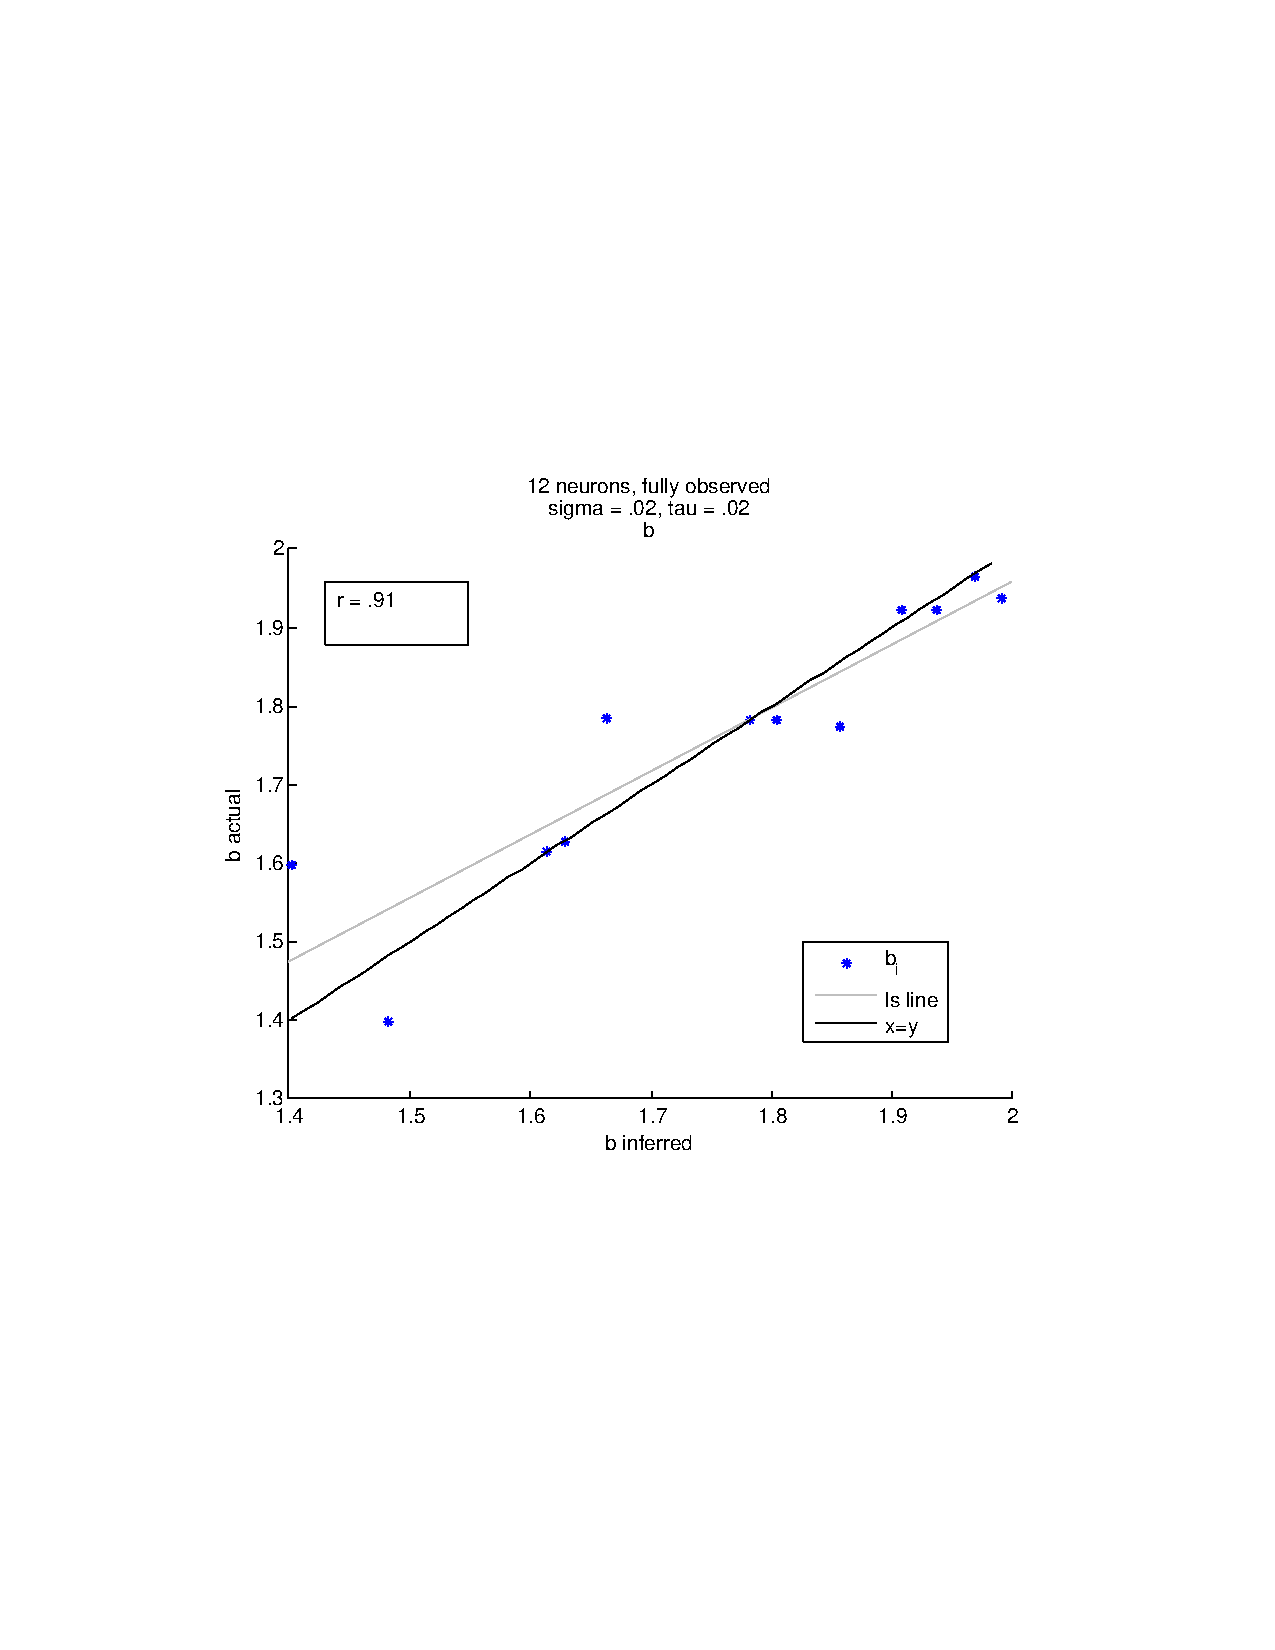
\includegraphics[width=0.48\textwidth, trim=40mm 80mm 40mm 40mm, clip]{12n_noise_b}
}
\subfigure[Connectivity Weights]{
  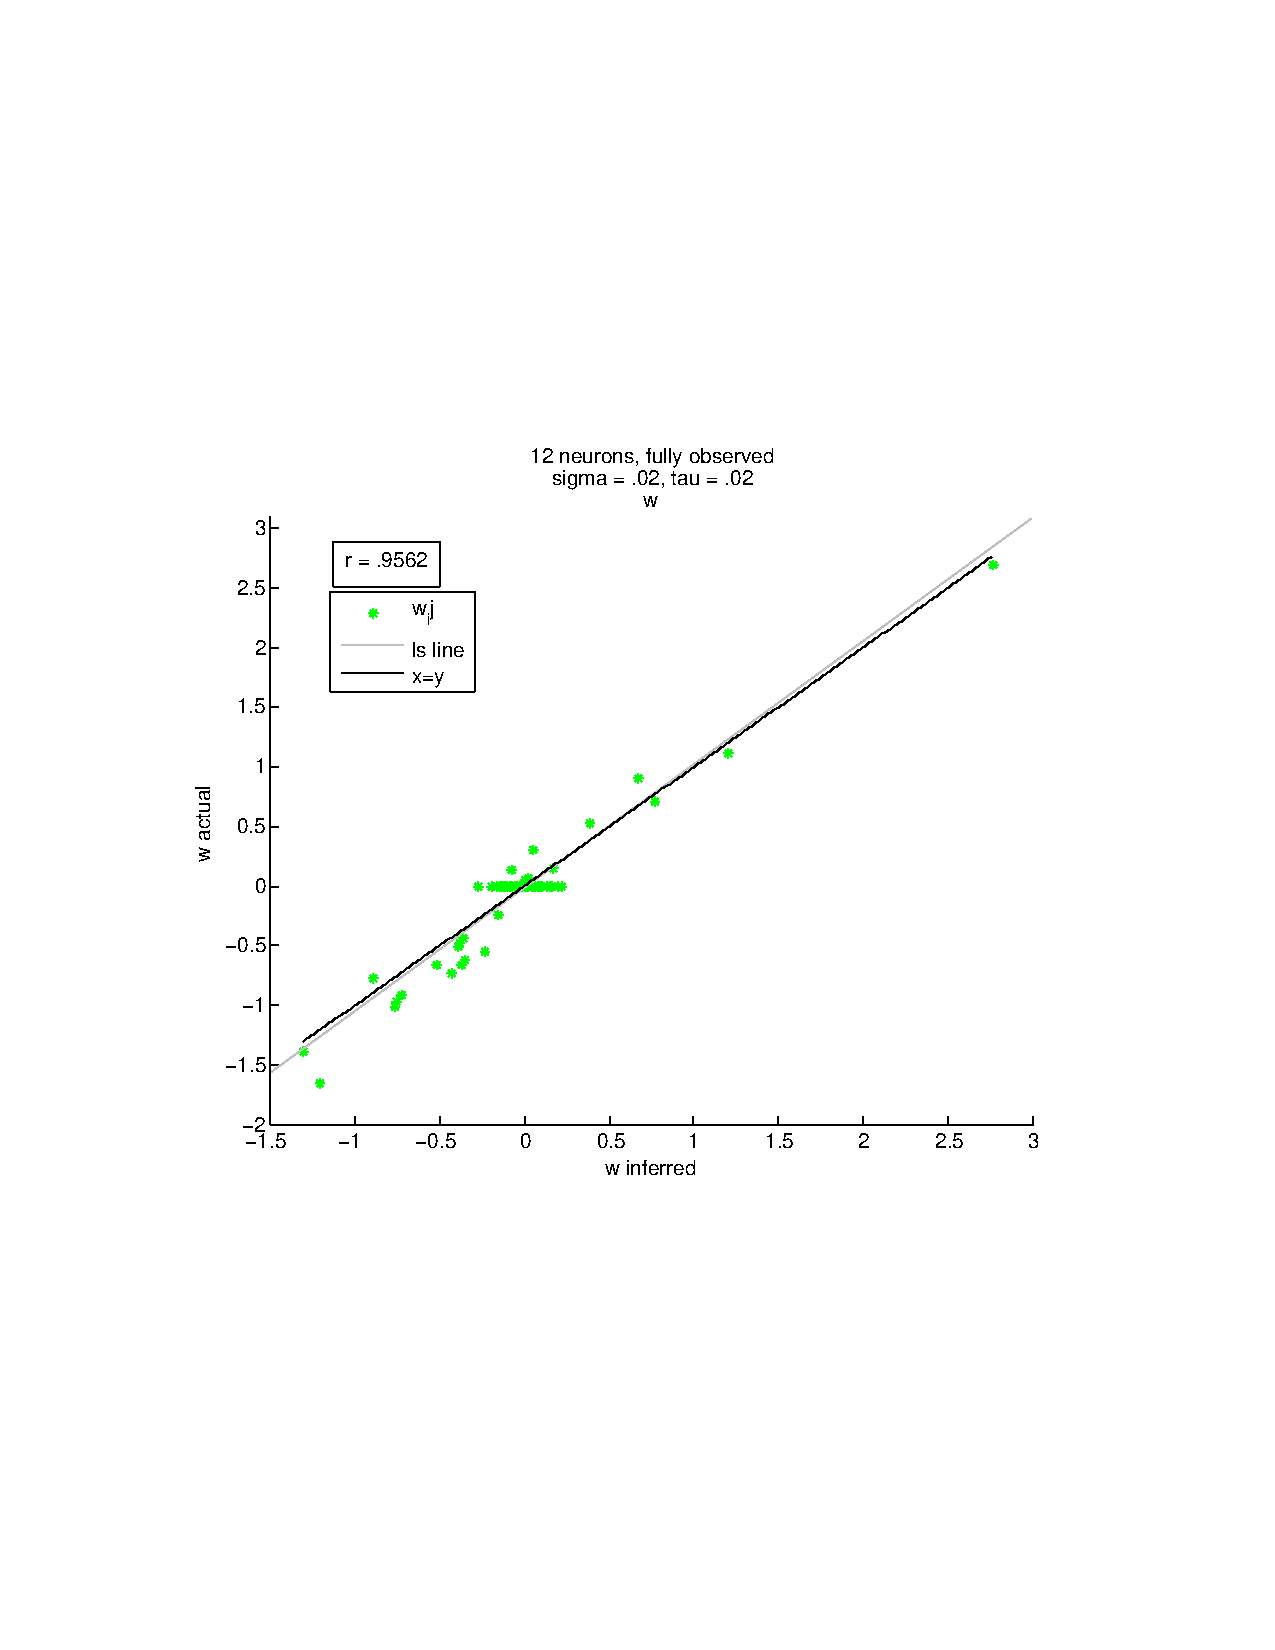
\includegraphics[width=0.48\textwidth, trim=40mm 80mm 40mm 40mm, clip]{12n_noise_w}
}
\caption{Inferred vs. true $b_i$ and $w_{ij}$ values for fully observed set of 12 neurons.}
\end{figure}

As shown in Figure~\ref{validation}, we were able to closely retrieve the parameters and therefore are confident that our algorithm works. However, it should be noted that here as well as in other experiments we generally underestimated inhibitory weights. This makes sense because firing is sparse in these networks and inferring inhibitory connections is dependent on coincident firing between an excitatory neuron, and inhibitory neuron, and a shared target neuron. Furthermore, it is difficult to determine an inhibitory weight unless a target neuron is firing tonically. Nonetheless, strong inhibitory connections are still well represented in our results.

\subsubsection{Indirect Weights}

\begin{figure}
\label{indirect}
\centering
\subfigure[Baselines]{
  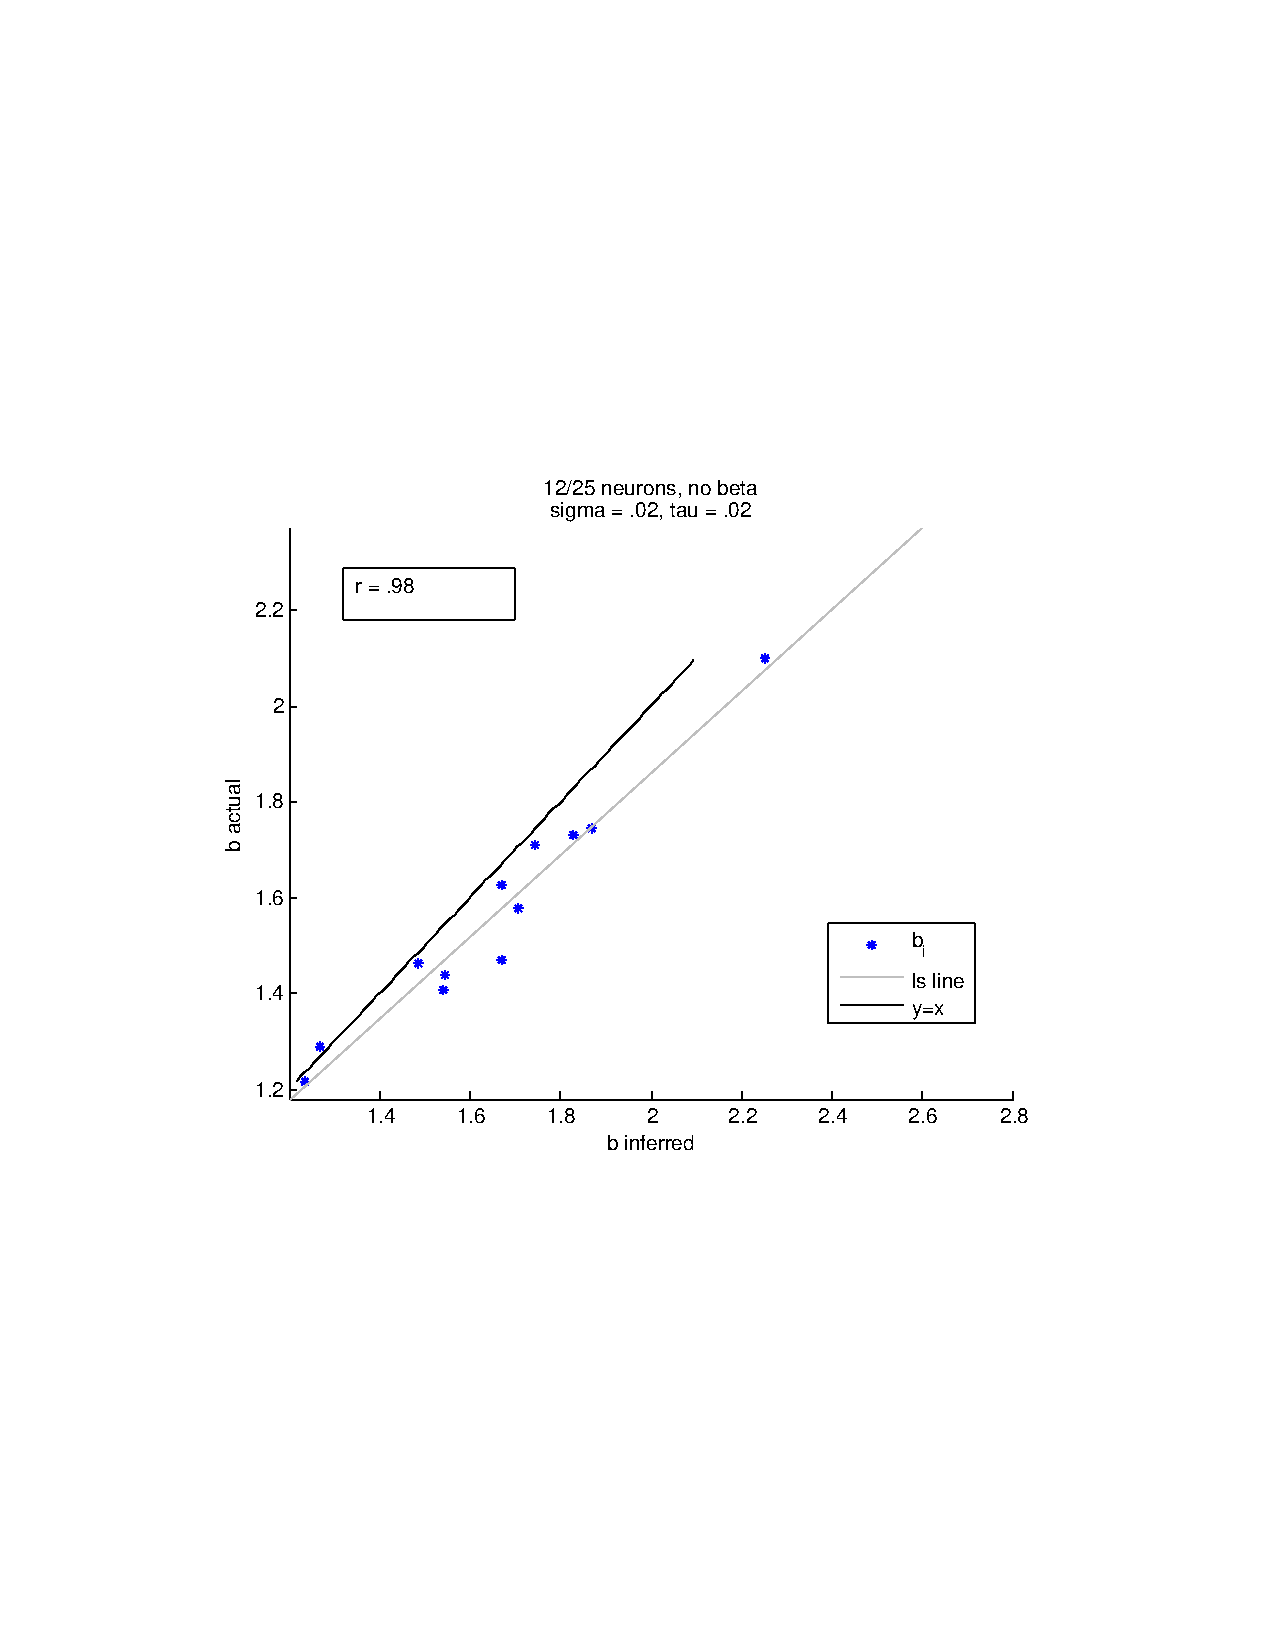
\includegraphics[width=0.48\textwidth, trim=40mm 80mm 40mm 40mm, clip]{25n_nobeta_b}
}
\subfigure[Connectivity Weights]{
  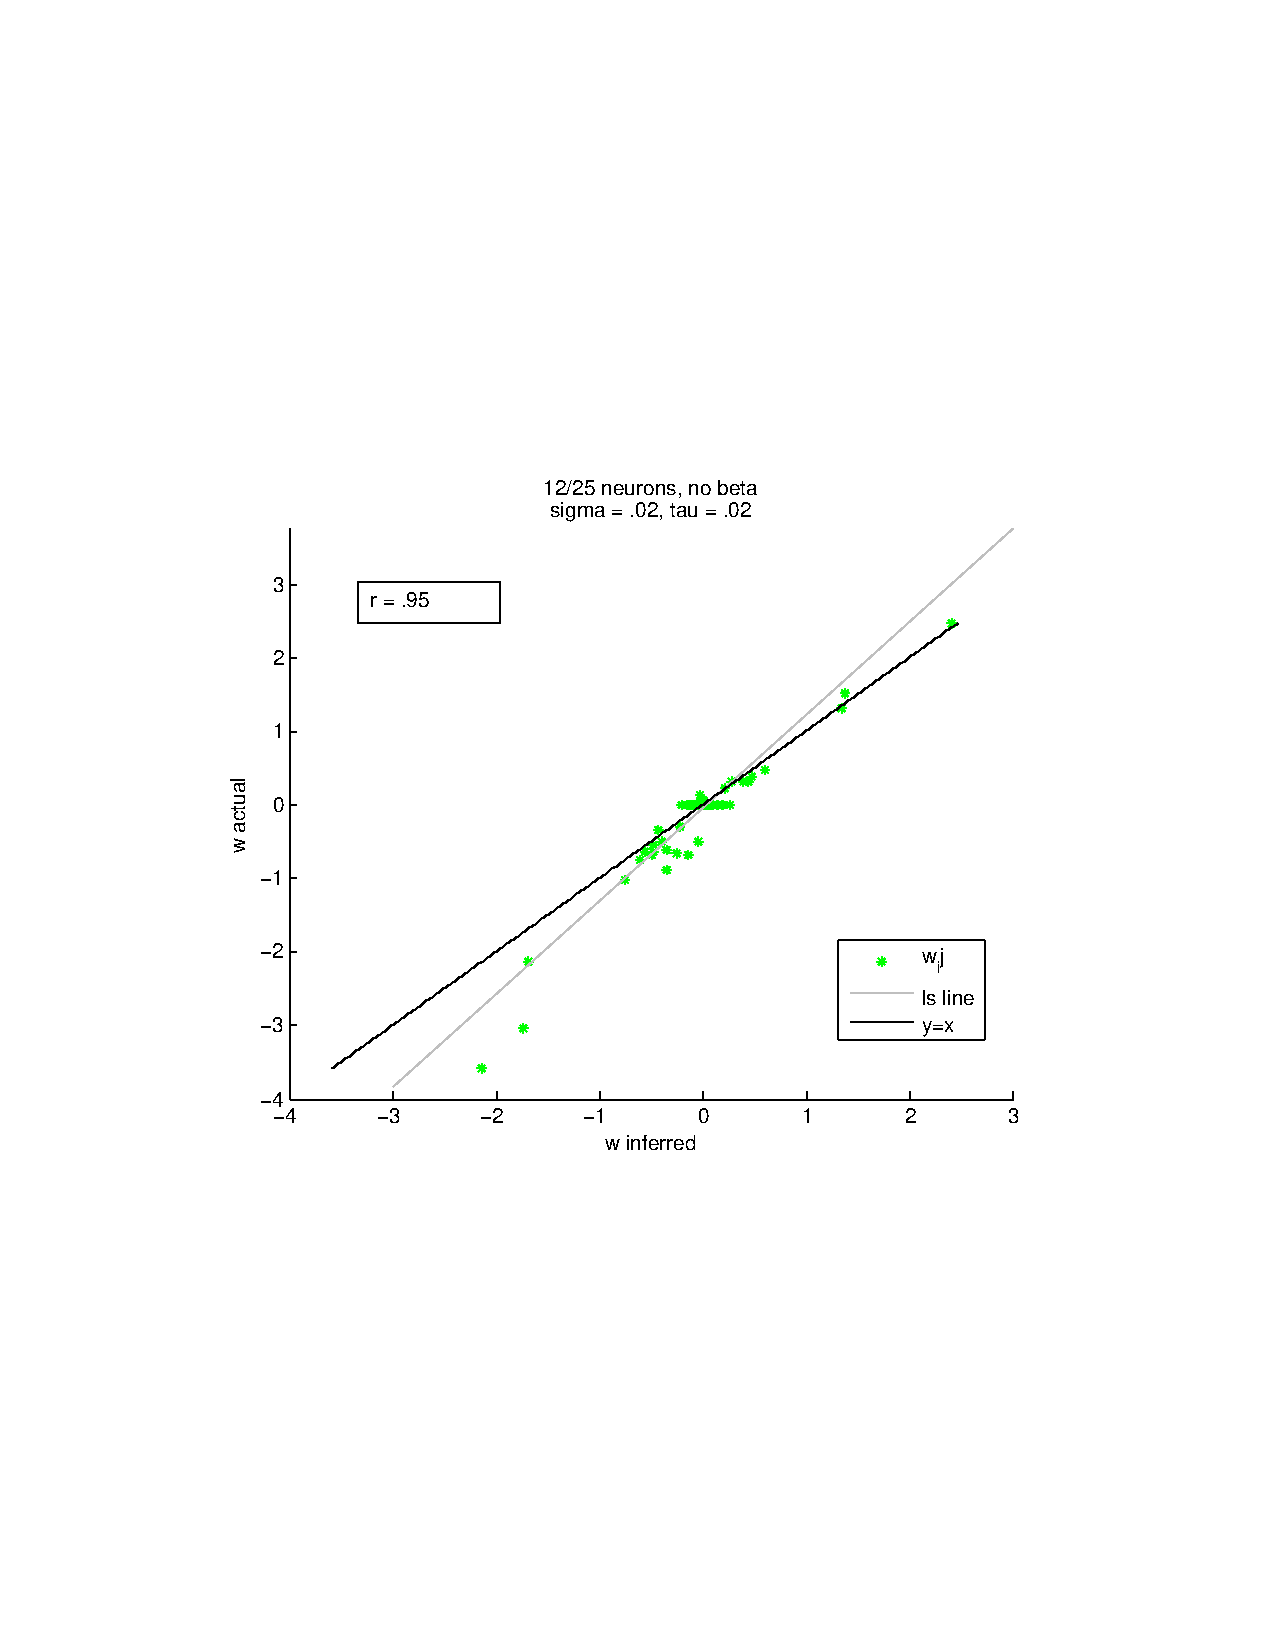
\includegraphics[width=0.48\textwidth, trim=40mm 80mm 40mm 40mm, clip]{25n_nobeta_w}
}
\subfigure[Baselines with Indirect Weights]{
  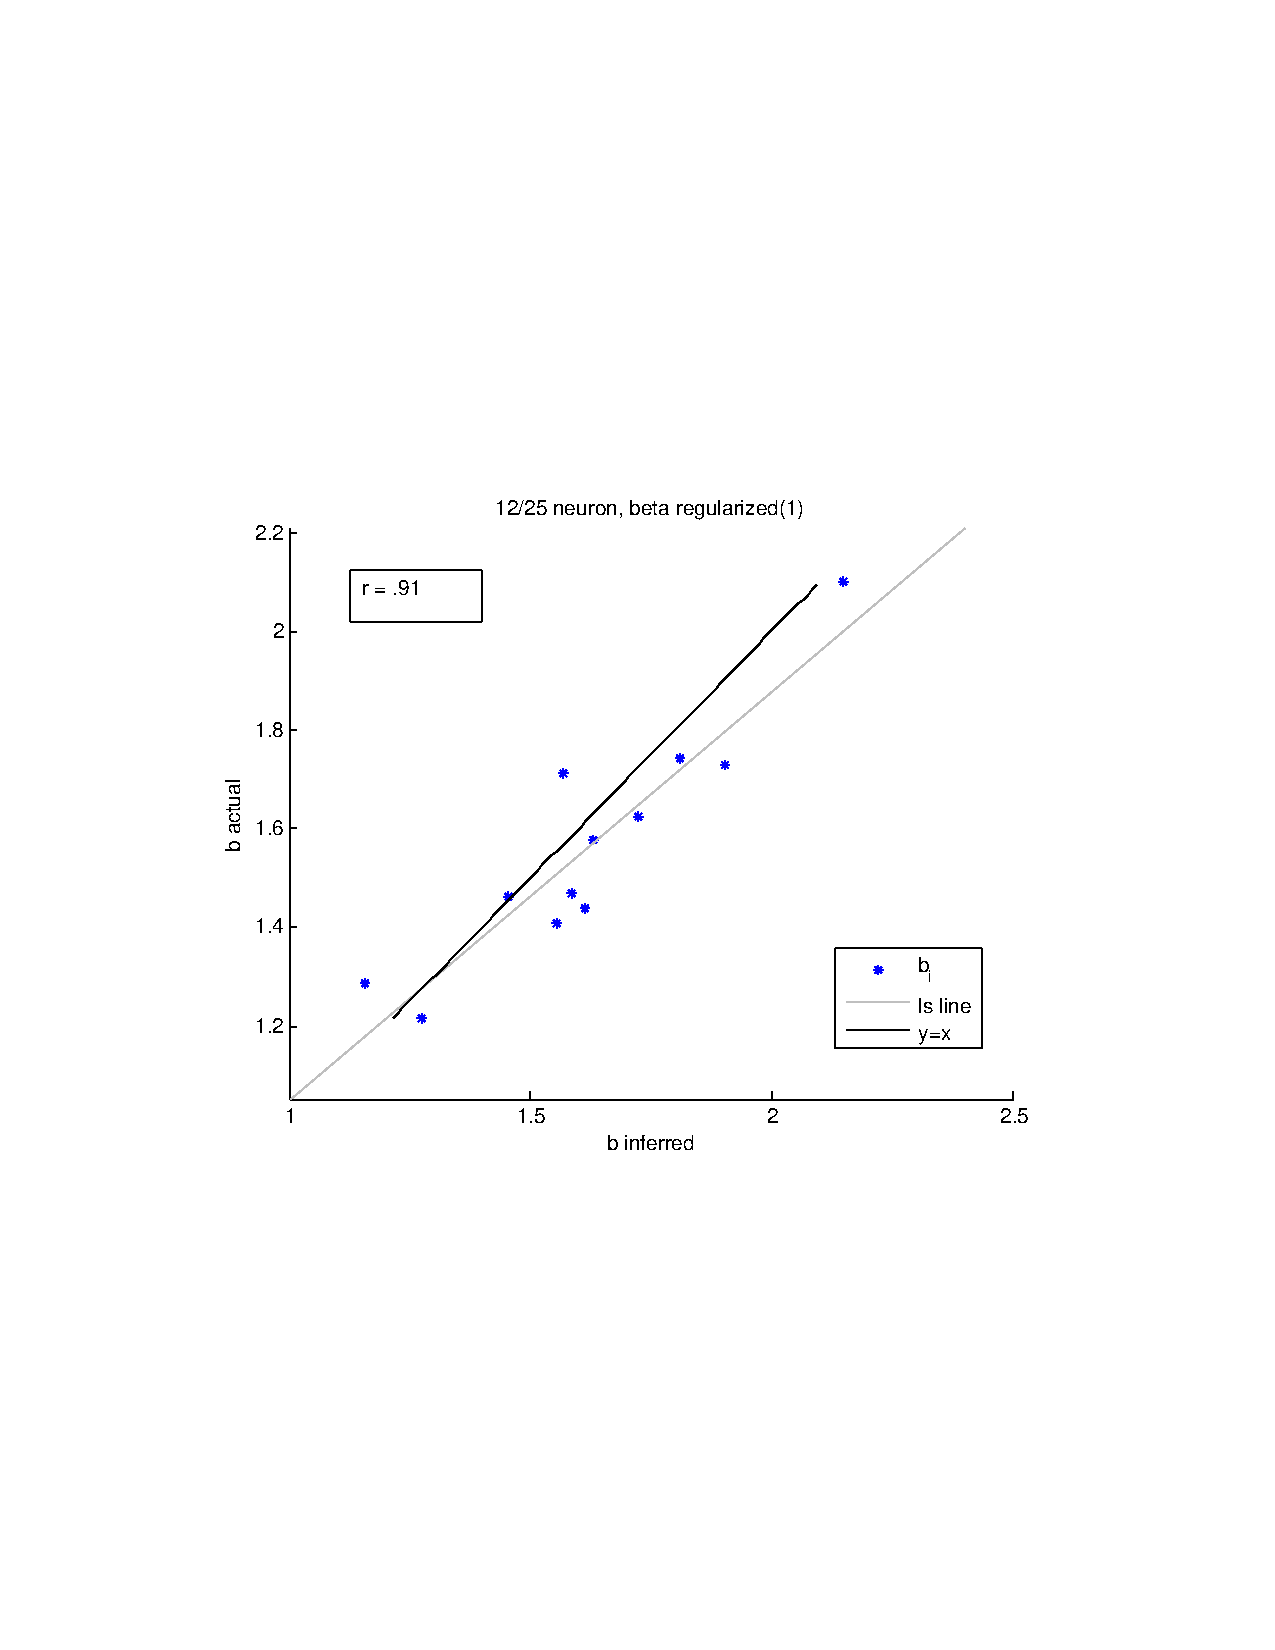
\includegraphics[width=0.48\textwidth, trim=40mm 80mm 40mm 40mm, clip]{25n_beta_b}
}
\subfigure[Connectivity Weights with Indirect Weights]{
  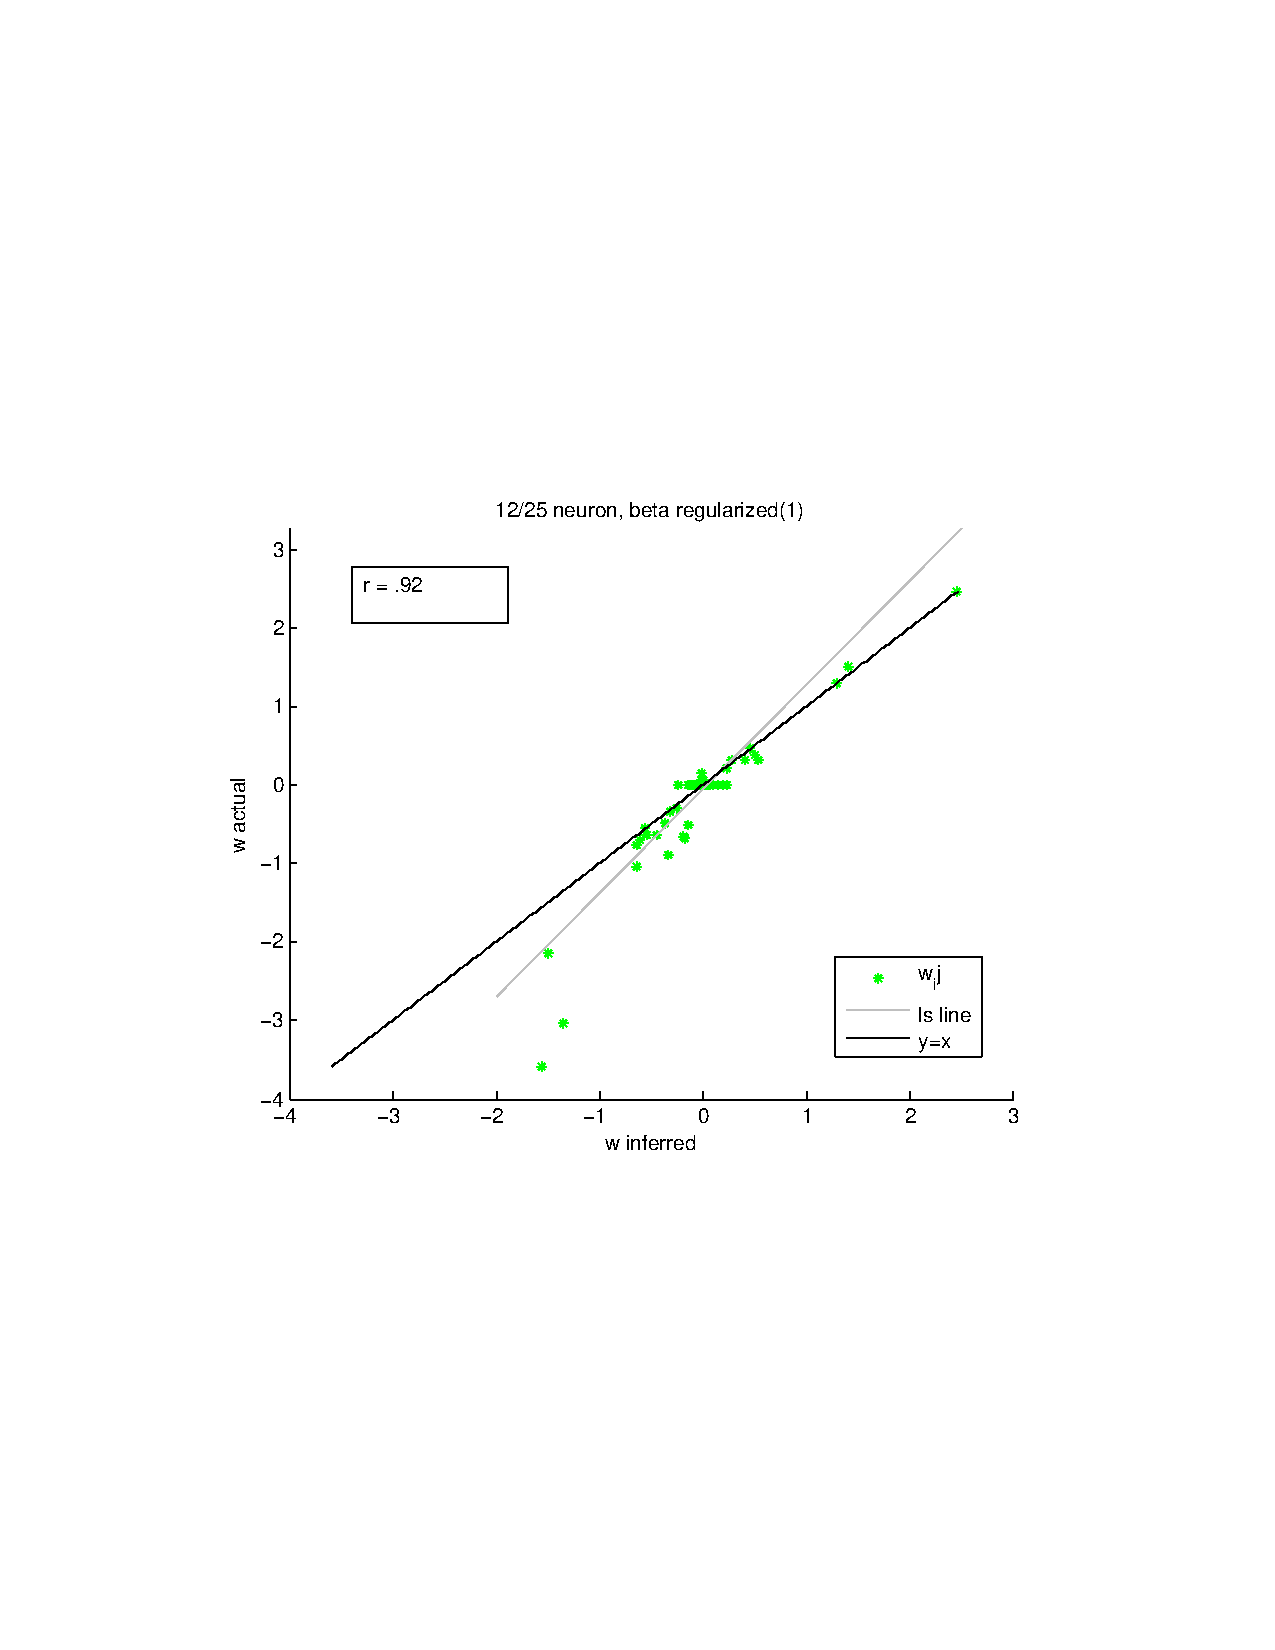
\includegraphics[width=0.48\textwidth, trim=40mm 80mm 40mm 40mm, clip]{25n_beta_w}
}
\caption{Inferred vs. true $b_i$ and $w_{ij}$ values for an observed set of 12 out of 25 total neurons. The top row shows inference without indirect weights. The bottom row shows the accuracy improvement when indirect weights are added to the model. See text for details.}
\end{figure}
In the case of simulated data, we have an interesting opportunity to test the quality of the indirect component of our model. We can simulate a large population neurons and only use a subset as the observed neurons in our model. We can then compare our inferred indirect weights with the known direct weights of the simulated data. Also, we can compare the results of the $\mathbf{b}$ and $W$ parameters of the same data with $\bm{\beta}$ inferred and not inferred.

When we performed inference on a subpopulation of 12 neurons (out of 25 total) and omitted the $\bm{\beta}$ parameters we still found a high correlation between the actual and inferred values of $\mathbf{b}$ and $W$, however we consistently overestimated the values of $\mathbf{b}$. When we included the $\bm{\beta}$ parameters, we found that the correlation remained more or less the same for both $\mathbf{b}$ and $W$, but we much more accurately inferred the $\mathbf{b}$ values \figref{indirect}. These results make sense because without indirect weights, any excitatory input into the system (excitatory inputs are more likely in our simulation and in actual nervous systems) would have to be summed into the $\mathbf{b}$ parameters. When we include indirect weights, these input can be put in their proper place, making estimations of $\mathbf{b}$ more accurate. 

We also designed a network such that there was a series of strong excitatory connections from an observed neuron, through several unobserved neurons, and back into the observed population.  When we performed inference over this network, we were able to find a relatively strong $\beta$ value that corresponded with part of this on the appropriate time scale. For example, the network contained the chain of weights $w_{13,4}=1.9$, $w_{1,13}=2.0$. This results on in indirect connection from neuron 4 to neuron 1 through the unobserved neuron 13. We found the corresponding values $\beta_{1,4,1}=.33$, $\beta_{1,4,2}=.34$, and $\beta_{1,4,3}=.17$. Compare these values to the average over $\beta_{1js}=.009$ and variance of .016.

However, we did not find a representative $\beta$ value in every instance where it would seem likely. This could either be a flaw in our model or a result of more complex interaction in the network that are difficult to analyze upon inspection. Also, the correlation of inferred to actual $\mathbf{b}$ values was lower than in most of our experiments, $r=.49$.

\subsubsection{Real Data}

When took spike trains recorded from 87 rat prefrontal cortex, binned them such that $\Delta = .010$ and performed inference over a subpopulation of 12 neurons. Our results here were more ambiguous, returning a handful of fairly weak inhibitory neurons among other neurons with no strong weights onto other observed neurons. For  $\bm{\beta}$, we found that $\beta_{max}=.1234$, $\beta_{min}=-.0594$, $\beta_{mean}=-.00062$, and $\beta_{var}=.0003$.

\section{Conclusions \& Future Directions}

While we feel confident that our algorithm and methodology are sound and we see some improvement in inference when we include $\bm{\beta}$, there is clearly more work to be done to fit indirect connectivity into the current model. Though we improved the $\mathbf{b}$ values, one would expect the values to be originally overestimated and then reduced instead of the opposite. This is because with indirect weights accounted for, their weights would have to be included in $\mathbf{b}$. We plan to look into this logic more in further experiments. Also, we would like to investigate creating a prior for $\bm{\beta}$ using methods similar to the pattern-growth algorithms used in \citep{patnaik2011}.



\begin{small}
\bibliographystyle{plainnat}
\bibliography{refs} 
\end{small}

\section*{Appendix}
\subsection{Hyperparameters}
We set $.02 \leq \sigma \leq .25$, $\tau = .02$ \citep{gerstner2002}, and $\Delta = .01$ for both the simulation and inference, though we did vary both $\sigma$ and $\tau$ and found our inference robust to those changes.
\subsection{Derivatives for M-step}
Evaluating $Q$ is expensive as it requires a complete pass over the
data---up to 15,000 timesteps. Analytical derivatives - the gradient and Hessian - are essential;
fortunately, they are not difficult to derive. Denote by
$\theta_1, \theta_2$ any scalar parameters. Then
\begin{align*}
\frac{\partial Q}{\partial \theta_1} &= \left(1 - n_i(t)\right) \left(-\exp{\left\{-e^{J_i(t)}\right\}} \Delta \frac{\partial J}{\partial \theta_1}\right) \\
    &+ n_i(t) \frac{\exp{ \left\{ -e^{J_i(t)} \Delta + J_i(t) \right\}} \Delta \frac{\partial J}{\partial_\theta1} }{1 - \exp{\left\{-e^{J_i(t)}\Delta\right\}}} \\
\frac{\partial^2 Q}{\partial \theta_1 \partial \theta_2} / \frac{\partial J}{\partial \theta_1} \frac{\partial J}{\partial \theta_2} &= \exp{\left\{-e^{J_i(t)\Delta} + J_i(t)\right\}}\Delta \\
 &+ \frac{\exp{\left\{-2e^{J_i(t)}\Delta + 2J_i(t)\right\}}\Delta^2}{1 - \exp{\left\{-e^{J_i(t)\Delta}\right\}}} \\
 &+ \exp{\left\{-e^{J_i(t)\Delta} + 2J_i(t)\right\}} \Delta^2 
\end{align*}
We omit the $\dfrac{\partial^2 J}{\partial \theta_1^2}$, since $J$
is linear in each variable, so the second derivatives are zero. To
compute both the gradient and Hessian, parameter, we simply multiply
the general forms above by each one of:
\begin{align}
\frac{\partial J_i(t)}{\partial b_i}         &= 1 \\
\frac{\partial J_i(t)}{\partial w_{ij}}      &= h_{ij}(t) \\
\frac{\partial J_i(t)}{\partial \beta_{ijs}} &= n_i(t - s)
\end{align}


\end{document}
